\documentclass[10pt]{article}
\usepackage{graphicx}
\usepackage{amssymb}
\usepackage{epstopdf}
\usepackage{enumitem}
\usepackage{multicol,multirow}
\DeclareGraphicsRule{.tif}{png}{.png}{`convert #1 `dirname #1`/`basename #1 .tif`.png}
\renewcommand{\tablename}{Tabla} 
\renewcommand{\figurename}{Figura} 
\newcommand*\circled[1]{\tikz[baseline=(char.base)]{\node[shape=circle,blue,draw,inner sep=2pt] (char) {#1};}}

% For a visual definition of these parameters, see
\textwidth = 6.5 in
\textheight = 9 in
\oddsidemargin = 0.0 in
\evensidemargin = 0.0 in
\topmargin = 0.0 in             
\headheight = 0.0 in            
\headsep = 0.0 in
            
\parskip = 0.2in                % vertical space between paragraphs
% Delete the % in the following line if you don't want to have the first line of every paragraph indented
%\parindent = 0.0in

\begin{document}
\begin{center}
    {\Large Certamen 3, Programaci\'on II} \\
    \emph{\small Prof. Rodrigo Olivares} \\
    \emph{\small Ayud. Diego Agullo} \\
    \emph{\scriptsize Julio 13, 2015}
\end{center}
\vspace*{-35pt}
\begin{center}
    \rule{1\textwidth}{.3pt}
\end{center}
\vspace*{-42pt}
\begin{center}
    \rule{1\textwidth}{2pt}
\end{center}

\vspace*{-15pt}
{\small \textbf{Instrucciones}:}
\vspace*{-15pt}

{\scriptsize
\begin{itemize}
    \item[-] El puntaje m\'aximo del certamen es 100\%, siendo el 60\% el m\'inimo requerido para aprobar.
    \item[-] Responda cada pregunta en la hoja indicada, agregando su nombre. Si no responde alguna pregunta, debe entregar la hoja con su nombre e indicar que \textbf{no responde}.
    \item[-] El certamen es \underline{\textbf{individual}}. Cualquier intento de copia, ser\'a sancionado con nota \textbf{1,0}.
\end{itemize}
\vspace*{10pt}

\vspace*{-30pt}

\begin{enumerate}

    \item \emph{30pts.} De las siguentes afirmaciones, encierre en un c\'irculo la o las alternativas correctas (\emph{3pts c/u}).
    \begin{multicols}{2}

    \begin{enumerate}[label=(\alph*)]
        \item[i.] Un thread: 
        \item Es un proceso que se ejecuta en memoria.
        \item Es un flujo de un proceso en memoria.
        \item Puede ser creado como clase en Java.
        \item Puede ser instanciado como objeto.
        \item Ninguna de las anteriores.
    \end{enumerate}

    \begin{enumerate}[label=(\alph*)]
        \item[ii.] Para construir una hebra se requiere:
        \item Extender de una s\'uper clase Thread.
        \item Implementar una interfaz Thread.
        \item Extender de una s\'uper clase Runneable.
        \item Implementar una interfaz Runneable.
        \item Utilizar el m\'etodo sleep. 
    \end{enumerate}

    \begin{enumerate}[label=(\alph*)]
        \item[iii.] Para una hebra o hilo se debe:
        \item Iniciar con el m\'etodo run.
        \item Iniciar con el m\'etodo start.
        \item Sobreescribir el m\'etodo run.
        \item Sobreescribir el m\'etodo start.
        \item Instanciar la hebra.
    \end{enumerate}

    \begin{enumerate}[label=(\alph*)]
        \item[iv.] En el ciclo de vida de una hebra, el estado: 
        \item New crea e inicializa la hebra.
        \item Runnable ejecuta la hebra, si hay tiempo CPU asignado.
        \item Blocked se ejecuta, sin importar estados internos.
        \item Dead es invocado generalmente por el m\'etodo stop.
        \item Yield, verifica el rendimiento del estado Runnable.
    \end{enumerate}

    \begin{enumerate}[label=(\alph*)]
        \item[v.] Un recurso compartido:
        \item Puede ser una clase.
        \item Puede ser un objeto de la clase.
        \item Puede ser un atributo de la clase.
        \item Siempre debe estar sincronizado.
        \item Debe ser declarado como private o protected.
    \end{enumerate}

    \begin{enumerate}[label=(\alph*)]
        \item[vi.] Los bloqueos de recursos compartidos se consiguen:
        \item Package, bloqueando los accesos a las clases internas.
        \item Clase, bloqueando m\'etodos y atributos de la clase.
        \item Atributo, declar\'andolos como static.
        \item Objeto, declarando los m\'etodos como synchronized.
        \item Ninguna de las anteriores
    \end{enumerate}

    \begin{enumerate}[label=(\alph*)]
        \item[vii.] Respecto a las interfaces gr\'afica en Java:
        \item Swing sustituye a AWT.
        \item AWT sustituye a Swing.
        \item AWT se apoya en Swing.
        \item AWT incopora los JComponents.
        \item Ninguna de las anteriores
    \end{enumerate}

    \begin{enumerate}[label=(\alph*)]
        \item[viii.] Referente a JFrame:
        \item Habitualmente se usa para crear la ventana principal.
        \item Su m\'etodo getPaneContent() obtiene el panel principal.
        \item Su m\'etodo add() permite agregar componentes al panel.
        \item Su m\'etodo size() permite dimensionar la ventana.
        \item Todas las anteriores
    \end{enumerate}

    \begin{enumerate}[label=(\alph*)]
        \item[ix.] Para realizar acciones desde un bot\'on Se requiere:
        \item Crear una clase que implemente un ActionEvent.
        \item Crear una clase que implemente un ActionList.
        \item Sobreescribir el m\'etodo actionList(ActionPerformance)
        \item Sobreescribir el m\'etodo actionPerformance(ActionEvent)
        \item Agregar la instancia de la clase oyente, al bot\'on.
    \end{enumerate}
    
    \begin{enumerate}[label=(\alph*)]
        \item[x.] Algunos JComponents : 
        \item JPane, JScrollPane, JDialog.
        \item JPanel, JScrollPanel, JDialogPane.
        \item JFileChooser, JScrollPane, JLabel.
        \item JList, JButton, JText.
        \item JPasswordField, JTextField, JTextArea.
    \end{enumerate}

\end{multicols}

\newpage

\item \emph{40pts.} Una importante empresa de retail le ha solicitado simular los procesos de ingreso y egreso de clientes a su tienda. Para ello, debe desarrollar una herramienta en Java que permita gestionar procesos concurrentes y mostrar el flujo de secuencia. Debe considerar los siguiente:

    \begin{enumerate}[label=(\alph*)]
        \item No es factible que egresen clientes si la tienda est\'a vac\'ia.
        \item No es factible que ingresen clientes, si la tienda est\'a llena (l\'imite de 100 clientes). 
        \item La cantidad de clientes que ingresan y egresan es aleatoria (n\'umero entero, mayor a cero y menor a 10).
        \item Existe un tiempo entre los cliente que ingresan y egresan (aleatorio, mayor o igual 1 y menor o igual a 5 segundos).
	\end{enumerate}

\newpage

\item \emph{30pts.} Desarrollar una herramienta, con interfaz de usuario en Java que permita transformar una palabra, frase u oraci\'on en c\'odigo morse y viceversa. Para ello, asuma que existe una clase llamada \textbf{TranslatorHelper} que pose\'e los m\'etodos est\'aticos \textbf{text2morse(String)} y \textbf{morse2text(String)} que transforma de texto a morse y de morse a texto, respectivamente. La interfaz de usuario debe contener al menos los componentes que se muestran en la Figura \ref{fig:graf-user-mt}.

    \begin{figure}[h]
        \begin{center}
            \fbox{\fbox{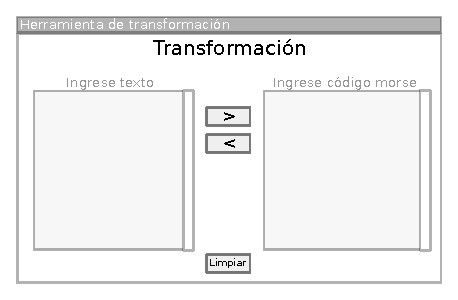
\includegraphics[scale=1]{images/fig-1.pdf}}}
            \caption{Interfaz de usuario}\label{fig:graf-user-mt}
        \end{center}
    \end{figure}


\end{enumerate}
}
\end{document} 
